\documentclass[11pt]{article}

% --- arXiv-friendly preamble (standard packages only) ----------------------
\usepackage[utf8]{inputenc}
\usepackage[T1]{fontenc}
\usepackage{lmodern}
\usepackage[margin=1in]{geometry}
\usepackage{amsmath,amssymb}
\usepackage{booktabs}
\usepackage{microtype}
\usepackage{listings}
\usepackage{xcolor}
\usepackage{pgfplots}
\pgfplotsset{compat=1.17}
\usepackage[hidelinks]{hyperref}

\lstset{basicstyle=\ttfamily\small,breaklines=true,frame=single,
        backgroundcolor=\color{gray!6},columns=fullflexible}

\title{\textbf{OctaSoma}: A Cache-Efficient 3-D Octree for Semantic Memory,\\
and the Limits of Ultra-Low-Dimensional Projection}

\author{OctaSoma Project\thanks{Author and affiliation to be set before
submission. Source, code, and reproduction harness: the project repository.}}

\date{June 2026}

\begin{document}
\maketitle

\begin{abstract}
Agent memories are usually opaque: an embedding is stored in a high-dimensional
vector index and recall is a black-box nearest-neighbour lookup. We take a
different stance. Building on the idea of projecting embeddings to three
dimensions and indexing them in an octree~\cite{octreerag}, we treat the octree
not as a flat index but as a \emph{fractal, multi-resolution memory}: because the
tree is self-similar at every scale, each depth is a \emph{zoom level}, so a query
can be answered -- and \emph{explained} -- at any resolution, from the broad theme
near the root to the exact recollection at a leaf. \textbf{OctaSoma} is a compact,
dependency-light, 100\% safe-Rust engine that realises this: a learned (PCA) or
deterministic (Johnson--Lindenstrauss) $3\times D$ projection, a bucket
point-region octree with 64-byte nodes, \emph{exact} branch-and-bound $k$-NN
(provably identical to brute force, $38$--$77\times$ faster than a linear scan),
zoomable multi-resolution recall, and -- because every memory carries real 3-D
coordinates -- \emph{native explainability and visualisation} that a
high-dimensional index cannot offer. We also measure, honestly, what three
dimensions cost. \emph{Exact} nearest-neighbour recall@1 collapses to
${\approx}0\%$, but \emph{topical} (cluster) recall is recoverable with PCA when a
corpus has few dominant themes ($100\%$ at four themes, $73\%$ at sixteen, $3\%$ at
$256$; random projection trails PCA $4$--$6\times$). A head-to-head comparison
against a full-dimensional exact store locates OctaSoma's niche as a compact,
explainable \emph{coarse router}: $85\times$ smaller coordinates and, used as a
pre-filter, ${\sim}93\%$ of the full-$D$ cluster recall at ${\sim}90\times$ lower
query cost. Finally, we frame OctaSoma as the \emph{semantic-spatial} function of a
three-part agent-memory stack: a causal memory narrows recall to a small region,
OctaSoma supplies the cheap, explainable semantic layer within it, and an attention
kernel consumes the result. Deployed \emph{per region} rather than as one global
index, this cascade retrieves the target on real agent-codebase data at $99\%$ hit
and ${\sim}26$ tokens per turn (${\sim}137\times$ fewer than injecting everything),
where OctaSoma's \emph{global} 3-D index alone scores $0\%$ -- the coarse router is
decisive only as one brick of the ensemble. Our contribution is the
multi-resolution, explainable memory model, its deployment as one function of an
inference pyramid, and an honest characterisation of its operating range, delivered
as a clean reproducible artifact -- not the underlying projection pipeline, which we
attribute to prior work~\cite{octreerag}.
\end{abstract}

\section{Introduction}
Embedding-based retrieval underpins modern semantic memory: text, images, or
agent observations are encoded as vectors in $\mathbb{R}^D$ (commonly
$D\in[128,4096]$), and relevance is approximated by nearest-neighbour search.
Production systems keep the full embedding and rely on approximate
nearest-neighbour (ANN) indexes such as HNSW~\cite{hnsw} or
IVF-PQ~\cite{ivfpq,faiss} to make that search tractable.

This paper takes that opposite extreme as a starting point and turns it into a
\emph{memory model}. Instead of preserving $D$ dimensions, we collapse the
embedding to \emph{three} and index it in an octree~\cite{octreerag}; but rather
than treat the tree as a flat nearest-neighbour index, we exploit its defining
property -- it is a \emph{fractal}, self-similar at every scale -- to expose the
whole hierarchy as a \emph{zoomable, multi-resolution memory}. Each depth is a
zoom level: a recall can be navigated from the broad theme near the root to the
exact memory at a leaf. Three dimensions are what make this work: a spatial octree
is natural, points are literally visualisable, recalls become \emph{explainable}
(every memory has real coordinates), and per-item storage is minimal. The question
is how much useful semantics such an aggressive bottleneck retains, and under what
conditions.

Our answer is empirical and two-sided. The index itself is excellent: exact,
fast, compact, and safe. The projection is the bottleneck, and we quantify it
precisely. The exact nearest neighbour of a high-$D$ embedding almost never
survives projection to 3-D (recall@1 $\approx 0\%$). Yet \emph{coarse topical
structure} does survive, provided (i) the projection is \emph{learned} (PCA, not
random) and (ii) the corpus has \emph{few dominant themes}. We give the decay
curve and a rule of thumb.

\paragraph{Contributions.}
\begin{enumerate}
  \item A \textbf{fractal, multi-resolution memory model}: every level of the
  octree is used as a zoom level, so a recall can be summarised and navigated from
  coarse theme to exact memory (\texttt{zoom}/\texttt{zoom\_path}). To our
  knowledge this navigable, multi-resolution use of a projected-embedding octree is
  new; the closest prior work~\cite{octreerag} uses the tree as a flat retrieval
  index.
  \item \textbf{Native explainability and visualisation}: because memories have
  real 3-D coordinates, a recall reports its ``why'' -- the query's position, the
  nested regions it falls through, and the nearest memories with distances -- and
  the store exports directly for a 3-D viewer.
  \item An \textbf{honest characterisation} of the 3-D projection (exact vs.\
  topical recall, intrinsic dimensionality, PCA vs.\ random, a label-aware variant)
  and a \textbf{head-to-head comparison} against a full-dimensional store that
  locates the compact-router / pre-filter niche, with a fully reproducible harness.
  \item \textbf{OctaSoma}, a 100\% safe-Rust (\texttt{\#![forbid(unsafe\_code)]})
  reference implementation: exact branch-and-bound 3-D $k$-NN, dynamic world
  growth, versioned LZ4 persistence, an agent kernel and CLI -- one runtime
  dependency.
  \item A \textbf{systems result}: OctaSoma as the semantic-spatial function of a
  three-part inference pyramid (causal $\rightarrow$ semantic $\rightarrow$
  attention). Deployed \emph{per causal region} (a sharded index), the
  otherwise-coarse 3-D router helps land the target at $99\%$ hit and ${\sim}26$
  tokens per turn on real agent-codebase data -- a cascade in which no single
  component suffices (Section~\ref{sec:pyramid}).
\end{enumerate}
We explicitly do \emph{not} claim the embeddings-to-3-D-octree pipeline as novel;
that is due to Ellendula and Bajaj~\cite{octreerag}.

\section{Related work}
\paragraph{Vector search and ANN.} Inverted-file and product-quantisation
indexes~\cite{ivfpq,faiss} and graph indexes such as HNSW~\cite{hnsw} dominate
high-dimensional retrieval. They operate in the original space (or a mildly
compressed one) and target high recall at large $D$. OctaSoma is not a competitor;
it occupies the opposite end of the dimensionality axis.

\paragraph{Dimensionality reduction.} The Johnson--Lindenstrauss
lemma~\cite{jl} guarantees that random linear maps approximately preserve pairwise
distances -- but only into dimensions logarithmic in the number of points, far
above three. Principal component analysis~\cite{pca} captures maximal-variance
directions; we extract the top three by power iteration with Hotelling
deflation~\cite{golubvanloan}. Non-linear methods (t-SNE~\cite{tsne},
UMAP~\cite{umap}) produce better 2-/3-D visualisations but are not single linear
maps and do not yield an exact, cheap online index; we deliberately restrict
ourselves to a linear $3\times D$ map.

\paragraph{Spatial indexes and data-oriented design.} Octrees and loose
octrees~\cite{octree,ulrich} are standard for 3-D point and region queries.
Branch-and-bound nearest-neighbour search with admissible bounds is classical for
$k$-d trees and their relatives~\cite{friedman}. Our implementation follows
data-oriented design~\cite{dod}: contiguous, index-referenced, POD nodes sized to
a cache line.

\paragraph{Low-dimensional projection with spatial trees.} Closest to our design,
Ellendula and Bajaj~\cite{octreerag} cluster sentence embeddings, project each
cluster to three dimensions, and maintain per-cluster dynamic octrees for hybrid
retrieval, reporting roughly $4.2\times$ faster queries than an inverted-file
index. OctaSoma shares this embeddings-to-3-D-octree pipeline; we do not claim it
as novel. We differ in scope and emphasis: a single \emph{global} PCA or JL map
(we measure PCA against JL), an exact, reproducible, dependency-light artifact
framed as agent memory, and an explicit account of \emph{when} the projection
fails and survives. Our recall/dimensionality findings match the broader ANN
literature~\cite{drsurvey}: aggressive reduction destroys exact-neighbour recall
while cluster membership stays meaningful~\cite{nnmeaning}, and axis-aligned space
partitions lose their advantage above roughly ten to twenty
dimensions~\cite{highdimann} -- which is exactly why an octree forces a projection
this aggressive.

\section{Method}
\subsection{Projection to $\mathbb{R}^3$}
An embedding $x\in\mathbb{R}^D$ is mapped by a row-major matrix
$W\in\mathbb{R}^{3\times D}$ to $p = Wx \in \mathbb{R}^3$. Each coordinate is a dot
product accumulated in \texttt{f64} over a fixed-order, 4-wide loop, making $p$
\emph{bit-identical across architectures} -- essential because the spatial layout,
and therefore every query answer, must be reproducible.

We provide two ways to obtain $W$:
\begin{itemize}
  \item \textbf{Johnson--Lindenstrauss (JL).} Fill $W$ from a seeded Xorshift64
  generator. Deterministic, instantaneous, data-independent.
  \item \textbf{PCA.} Centre a calibration matrix and extract its top-3 principal
  components by power iteration with Hotelling deflation, in \texttt{f64}.
\end{itemize}
In both cases the three rows are $L_2$-normalised. For a unit-norm embedding this
bounds every coordinate to $[-1,1]$ by Cauchy--Schwarz, so a unit world cube
already contains normalised data.

\subsection{Bucket point-region octree}
Points are indexed by an octree stored as a contiguous \texttt{Vec} of 64-byte
nodes referenced by \texttt{u32} indices (no pointers, no \texttt{unsafe}):
\begin{lstlisting}
struct OctreeNode {       // exactly 64 bytes = 1 cache line
  center:    [f32; 3],    // cube centre
  half_size: f32,         // half the edge length
  children:  [u32; 8],    // octant children, NONE = absent
  bucket_id: u32,         // leaf bucket index, NONE = internal
  _padding:  [u8; 12],
}
\end{lstlisting}
A node is a \emph{leaf} (owning a list of item ids in a side array
\texttt{leaf\_buckets}) or \emph{internal} (routing through \texttt{children}).
Keeping item lists out of the node keeps traversal to one cache line per node.

\paragraph{Insertion.} To insert $p$, we descend from the root following the
octant of $p$ (bit $i$ set iff $p_i \ge c_i$). At a leaf with spare capacity we
append; a full, still-divisible leaf is \emph{subdivided} (converted to internal,
its bucket redistributed into eight octant children) and the descent continues.
Because each subdivision exactly tiles a cube into octants and $p$ is guaranteed
inside the root cube, containment is preserved at every level -- the invariant the
search relies upon. Bit-identical points share a leaf bucket (a growable vector),
so nothing is ever dropped.

\paragraph{Dynamic world.} If an incoming coordinate exceeds the current
half-edge, the origin-centred root cube \emph{doubles} until it fits and the tree
is rebuilt from the stored points. Doubling makes growth geometric, hence
amortised $O(1)$ per insert; for normalised embeddings it never triggers.

\subsection{Exact $k$-nearest-neighbour search}
Given a query point $q$, \texttt{nearest}$(q,k)$ runs branch-and-bound:
visit a node, and at an internal node recurse into existing children ordered by
the lower bound
\begin{equation}
\underline{d}^2(q,\text{cube}) \;=\; \sum_{a\in\{x,y,z\}} \big(\max(0,\,|q_a-c_a|-h)\big)^2,
\end{equation}
the squared distance from $q$ to the nearest point of a child cube (0 if inside),
\emph{pruning} any child whose bound already exceeds the current $k$-th best
distance. Since the bound is admissible, no true neighbour is ever discarded:
\texttt{nearest} is \emph{exact} -- bit-identical to brute force -- and our test
suite asserts this over thousands of random points. Top-1 and top-$k$ payload
lookups wrap this primitive.

\subsection{Persistence and implementation}
The engine serialises to a versioned, little-endian \texttt{FRAC} v3 file whose
payload arena is LZ4-compressed; the loader validates magic, version, and
dimensionality before allocating, and never panics on malformed input. The whole
crate is safe Rust with a single dependency (an LZ4 codec); nodes are POD, the
RNG and PCA are dependency-free, and projection is deterministic across platforms.

\section{Evaluation}
\label{sec:eval}
\subsection{Setup}
We generate $N$ unit-norm embeddings in $\mathbb{R}^D$ from $C$ latent clusters
(``themes''): each sample is a random cluster centre plus renormalised
Gaussian-ish noise, giving a controllable intrinsic dimensionality via $C$.
Queries are a \emph{held-out} set from the same clusters with an independent noise
stream (querying inserted points would render recall@1 a trivial $100\%$). Ground
truth is the exact nearest neighbour in the \emph{full} $D$-dimensional space, by
brute force. We report: \emph{exact recall@}$k$ (true high-$D$ neighbours
recovered by the 3-D index), \emph{cluster recall@}$k$ (returned items in the
query's theme -- the metric topical memory needs), query latency (octree vs.\
brute-force over the same 3-D points; both exact), insertion throughput, and LZ4
ratio. All figures are single-machine, release-build, and reproducible via the
bundled harness.

\subsection{Results}
Table~\ref{tab:scale} reports the large-scale operating point. The octree $k$-NN
is exact and $67$--$77\times$ faster than a linear 3-D scan; PCA reaches $70.8\%$
cluster recall@1 where a random projection manages only $13\%$; \emph{exact}
recall@1 is $\approx 0\%$ for both. Payloads compress $5.5\times$.

\begin{table}[t]
\centering
\caption{Scale: $N{=}50{,}000$, $D{=}256$, $C{=}16$ themes, $k{=}10$.
Latency/throughput are machine-dependent.}
\label{tab:scale}
\begin{tabular}{lcccccc}
\toprule
Projection & cluster@1 & recall@1 & octree $k$-NN & brute 3-D & speed-up & inserts/s \\
\midrule
PCA (learned) & \textbf{70.8\%} & 0.0\% & 5.69\,\textmu s & 383.6\,\textmu s & 67$\times$ & 1.86\,M \\
JL (random)   & 13.0\%          & 0.0\% & 5.12\,\textmu s & 393.6\,\textmu s & 77$\times$ & 1.53\,M \\
\bottomrule
\end{tabular}
\end{table}

Figure~\ref{fig:sweep} and Table~\ref{tab:sweep} show how cluster recall depends
on intrinsic dimensionality ($N{=}20{,}000$, $D{=}128$). PCA preserves topical
structure perfectly for a few themes and decays as themes multiply; three
principal axes can separate only a handful of well-spread modes. JL trails badly
throughout.

\begin{table}[t]
\centering
\caption{Cluster recall@1 vs.\ number of latent themes ($N{=}20{,}000$, $D{=}128$,
$k{=}10$). Exact recall@1 stays $\approx 0\%$ everywhere.}
\label{tab:sweep}
\begin{tabular}{lcccc}
\toprule
themes $C$ & 4 & 16 & 64 & 256 \\
\midrule
PCA & \textbf{100.0\%} & \textbf{73.2\%} & 20.6\% & 2.6\% \\
JL  & 33.2\%           & 12.8\%          & 4.2\%  & 1.2\% \\
\bottomrule
\end{tabular}
\end{table}

\begin{figure}[t]
\centering
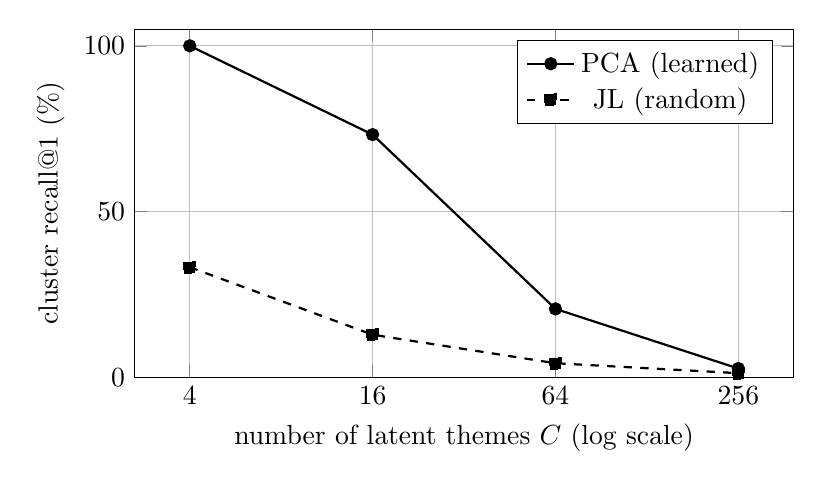
\begin{tikzpicture}
\begin{semilogxaxis}[
  width=0.82\linewidth, height=6cm,
  xlabel={number of latent themes $C$ (log scale)},
  ylabel={cluster recall@1 (\%)},
  xtick={4,16,64,256}, xticklabels={4,16,64,256},
  ymin=0, ymax=105, log basis x=2,
  legend pos=north east, grid=major]
\addplot[mark=*,thick] coordinates {(4,100.0)(16,73.2)(64,20.6)(256,2.6)};
\addplot[mark=square*,thick,dashed] coordinates {(4,33.2)(16,12.8)(64,4.2)(256,1.2)};
\legend{PCA (learned), JL (random)}
\end{semilogxaxis}
\end{tikzpicture}
\caption{Topical recall degrades with intrinsic dimensionality. A learned (PCA)
projection vastly outperforms a random (JL) one, but both collapse once the
corpus has more than a handful of dominant themes.}
\label{fig:sweep}
\end{figure}

\subsection{Analysis}
Four findings stand out. (1) \textbf{The index is exact and fast}: pruning yields
$38$--$77\times$ over a linear scan and the margin grows with $N$. (2)
\textbf{Three dimensions destroy exact neighbours}: recall@1 $\approx 0\%$ is
intrinsic to the projection, not the index. (3) \textbf{Topical structure can
survive}, but only under a learned projection and low intrinsic dimensionality.
(4) \textbf{PCA $\gg$ JL} for this task by $4$--$6\times$; if a calibration pass is
affordable, it is always worth it.

\section{Discussion: when three dimensions are enough}
OctaSoma is best understood as a \emph{coarse semantic router}. With a PCA
projection it reliably retrieves topically-relevant memories when a corpus has
roughly a dozen or fewer dominant themes -- a regime that covers many practical
agent-memory settings (a small set of personas, tasks, or domains), explainable
or visualisable indexing (points are literally 3-D), compact embeddable storage,
and coarse pre-filtering ahead of a heavier retriever. It is a poor fit for
general high-recall search over diverse corpora, where a full-dimensional ANN is
the right tool.

\section{OctaSoma as one function of an inference pyramid}
\label{sec:pyramid}
The honest verdict of Section~\ref{sec:eval} -- a single \emph{global} 3-D index is
a coarse router whose exact recall collapses as a corpus diversifies -- is not the
end of the story but a deployment instruction. OctaSoma is designed as the
\emph{semantic-spatial} layer of a three-function agent-memory stack, each function
owning a different kind of memory:
\begin{itemize}
  \item \textbf{Causal / structural} (long-term): a code/event graph that knows
  \emph{what depends on what}, but recalls lexically rather than semantically.
  \item \textbf{Semantic / spatial} (long-term): OctaSoma -- cheap, explainable,
  visualisable embedding recall.
  \item \textbf{Compressed working memory / attention} (short-term): a quantised
  KV-cache kernel that scores cached tiles for attention.
\end{itemize}
The causal and attention layers are companion systems in the same
stack.\footnote{CCOS (causal) and SLHAv2 (attention); see the project
repositories. This paper's contribution is OctaSoma and its role in the cascade,
not those systems.} CCOS itself states that its task recall is ``a deliberately
simple lexical entry point\,\dots\ not a semantic retriever'' -- precisely the gap
OctaSoma fills.

\paragraph{Per-region deployment.} Section~\ref{sec:eval} shows the global 3-D
index fails at scale. The remedy is to \emph{shard} it: keep one small OctaSoma
index per causal region (e.g.\ a source file) instead of a single global one. The
causal layer narrows a query to its region (small $N$); OctaSoma then ranks
\emph{within} that region, where three dimensions suffice. We implement this as a
sharded memory with a per-region PCA projection (a few lines over the core engine).

\paragraph{The cascade, measured.} Table~\ref{tab:cascade} runs the stack on
$795$ nodes of a real agent codebase, with held-out natural-language queries
embedded by a $768$-dimensional model. Read honestly:
\begin{itemize}
  \item \textbf{The ensemble is decisive; no single brick suffices.} Naive
  injection is wasteful ($3622$ tokens, $3\%$ relevant); OctaSoma's global 3-D
  alone is $0\%$; the causal region alone is correct but heavier. The cascade --
  causal narrowing then an exact rerank within the small region -- hits the target
  $99\%$ of the time at ${\sim}26$ tokens per turn, ${\sim}137\times$ fewer than
  naive, with fully causally-relevant context.
  \item \textbf{OctaSoma is the coarse layer, not the precise retriever.} The hit
  is landed by causal narrowing plus the exact rerank; OctaSoma's defensible role
  is the cheap, compact, explainable, visualisable coarse layer that proposes and
  organises -- consistent with Section~\ref{sec:eval}, not in tension with it.
\end{itemize}

\begin{table}[t]
\centering
\caption{The cascade on real data: $795$ nodes from a production agent codebase
(CCOS source), $763$ held-out queries, embedded with a $768$-dimensional model
(\texttt{nomic-embed-text}). ``Causal-relevant'' is the fraction of returned
context lying in the query's causal region; tokens are per turn.}
\label{tab:cascade}
\begin{tabular}{lccc}
\toprule
strategy & tokens/turn & target hit & causal-relevant \\
\midrule
naive (inject everything)               & 3622        & 100\%         & 3\%            \\
semantic-only (OctaSoma global 3-D)     & 30          & \textbf{0\%}  & 4\%            \\
causal-only (CCOS region)               & 158         & 100\%         & 100\%          \\
\textbf{causal + semantic (per region)} & \textbf{26} & \textbf{99\%} & \textbf{100\%} \\
\bottomrule
\end{tabular}
\end{table}

\paragraph{Visualising the attention kernel.} OctaSoma also serves the
working-memory kernel as a \emph{lens}, not a router: projecting $128$-dimensional
KV-cache tile latents to 3-D yields a navigable, head-coloured map of the cache,
exposing tile clusters and compression structure. We verified that this 3-D
pre-filter recovers only a fraction of the \emph{exact} attention top-$k$, so the
honest value here is inspection and diversity -- not attention selection, which the
kernel's own scoring owns.

\section{A high-precision tier: SimHash sketches}
\label{sec:sketch}
The 3-D projection is a coarse router by construction; where exact-neighbour
precision is needed we add a cheap, \emph{non-projective} tier rather than a
non-linear projection (which would forfeit the exact, incremental, explainable
index and still not preserve fine angles in three dimensions). A SimHash
sketch~\cite{simhash} of the \emph{full} embedding -- $b$ random hyperplanes, one
sign bit each -- turns cosine similarity into Hamming distance
($\mathbb{E}[\text{Hamming}]/b \approx \theta/\pi$), evaluated by a single
population count. Ranking by Hamming preserves far more angular structure than
three coordinates; used as a \emph{shortlist} before an exact cosine rerank over
stored embeddings, it recovers most of the true neighbours the projection discards,
at a fraction of a brute-force scan. Table~\ref{tab:sketch} reports recall@$M$ (the
exact nearest within a method's $M$ cheapest candidates; the hybrid's recall@1
equals recall@$M$ for a shortlist of $M$) on the data of Section~\ref{sec:eval}.

\begin{table}[t]
\centering
\caption{Recall@$M$ vs.\ the exact full-$D$ nearest neighbour ($N{=}20{,}000$,
$D{=}768$, $16$ themes). 3-D is bits-independent; a SimHash recall@$M$ is the
hybrid's recall@1 at shortlist $M$.}
\label{tab:sketch}
\begin{tabular}{lcccc}
\toprule
method & @1 & @32 & @128 & @512 \\
\midrule
3-D PCA (octree) & 0.0\% & 3.0\% & 10.7\% & 46.7\% \\
SimHash-256 & 1.7\% & 12.0\% & 30.7\% & 70.3\% \\
SimHash-512 & 1.7\% & 17.0\% & 40.0\% & 82.3\% \\
SimHash-1024 & 1.7\% & 21.7\% & \textbf{52.7\%} & \textbf{88.7\%} \\
\bottomrule
\end{tabular}
\end{table}

Two knobs trade precision for cost -- the sketch width $b$ and the shortlist size
$M$ (the rerank is one stored-embedding dot product per candidate). The tier is
$100\%$ safe, stable Rust (a dot product, a sign, and \texttt{u64::count\_ones}); it
trades memory for precision and \emph{complements} the 3-D layer, which remains the
cheap, explainable, visualisable router. It is also the precise \emph{global}
retriever of the pyramid (Section~\ref{sec:pyramid}) when a query has no causal
region.

\section{Limitations}
The projection is linear by construction; non-linear manifold learning could lift
topical recall but would forfeit the exact, cheap online index. Our clusters use
isotropic noise and are friendlier than real embedding manifolds, so cluster-recall
figures are an optimistic bound. Latency and throughput are single-machine and
single-thread. The engine is currently insertion-only (no deletion or TTL), and
mutation takes \texttt{\&mut self}, leaving concurrency policy to the caller.

\section{Conclusion}
We presented OctaSoma, a small, exact, safe-Rust 3-D octree for semantic memory,
and used it to measure the most extreme point of the dimensionality/fidelity
trade-off. The spatial index is exact, fast, and compact; the 3-D projection is
the limiting factor, erasing exact neighbours but -- under PCA and low intrinsic
dimensionality -- retaining useful topical structure. The honest takeaway is a
rule of thumb rather than a leaderboard win: collapse to three dimensions only
when your corpus is thematically narrow, learn the projection, and treat the
result as a coarse router. Its strongest use, accordingly, is not standalone but as
one function of an inference pyramid: sharded per causal region, the coarse router
becomes decisive -- $99\%$ recall at ${\sim}26$ tokens per turn on real data --
because a causal memory narrows the problem and an exact rerank finishes it. Code
and the full reproduction harness accompany this paper.

\begin{thebibliography}{99}
\bibitem{hnsw} Y.~Malkov and D.~Yashunin. Efficient and robust approximate nearest
neighbor search using Hierarchical Navigable Small World graphs. \emph{IEEE TPAMI},
2020.
\bibitem{ivfpq} H.~J\'egou, M.~Douze, and C.~Schmid. Product quantization for
nearest neighbor search. \emph{IEEE TPAMI}, 2011.
\bibitem{faiss} J.~Johnson, M.~Douze, and H.~J\'egou. Billion-scale similarity
search with GPUs. \emph{IEEE Trans.\ Big Data}, 2021.
\bibitem{jl} W.~Johnson and J.~Lindenstrauss. Extensions of Lipschitz mappings into
a Hilbert space. \emph{Contemp.\ Math.}, 1984.
\bibitem{pca} I.~T.~Jolliffe. \emph{Principal Component Analysis}. Springer, 2002.
\bibitem{golubvanloan} G.~Golub and C.~Van~Loan. \emph{Matrix Computations}. Johns
Hopkins University Press, 4th ed., 2013.
\bibitem{tsne} L.~van~der~Maaten and G.~Hinton. Visualizing data using t-SNE.
\emph{JMLR}, 2008.
\bibitem{umap} L.~McInnes, J.~Healy, and J.~Melville. UMAP: Uniform Manifold
Approximation and Projection. \emph{arXiv:1802.03426}, 2018.
\bibitem{octree} D.~Meagher. Geometric modeling using octree encoding.
\emph{Computer Graphics and Image Processing}, 1982.
\bibitem{ulrich} T.~Ulrich. Loose octrees. In \emph{Game Programming Gems}, 2000.
\bibitem{friedman} J.~Friedman, J.~Bentley, and R.~Finkel. An algorithm for finding
best matches in logarithmic expected time. \emph{ACM TOMS}, 1977.
\bibitem{dod} R.~Fabian. \emph{Data-Oriented Design}. 2018.
\bibitem{octreerag} A.~S.~Ellendula and C.~Bajaj. Self-Balancing, Memory-Efficient,
Dynamic Metric-Space Data Maintenance for Rapid Multi-Kernel Estimation. In
\emph{ECML-PKDD}, 2025. arXiv:2504.18003.
\bibitem{simhash} M.~S.~Charikar. Similarity estimation techniques from rounding
algorithms. In \emph{Proc.\ STOC}, 2002.
\bibitem{drsurvey} Dimensionality-reduction techniques for approximate nearest
neighbour search: a survey and evaluation. \emph{arXiv:2403.13491}, 2024.
\bibitem{nnmeaning} K.~Beyer, J.~Goldstein, R.~Ramakrishnan, and U.~Shaft. When is
``nearest neighbor'' meaningful? In \emph{ICDT}, 1999.
\bibitem{highdimann} W.~Li, Y.~Zhang, Y.~Sun, et al. Approximate nearest neighbor
search on high-dimensional data --- experiments, analyses, and improvement.
\emph{IEEE TKDE}, 2020.
\end{thebibliography}

\end{document}
